\documentclass[conference]{IEEEtran}
\IEEEoverridecommandlockouts
\usepackage{cite}
\usepackage{amsmath,amssymb}
\usepackage{graphicx}
\usepackage{booktabs}
\usepackage{array}
\usepackage{tikz}
\usetikzlibrary{arrows.meta,positioning,fit,backgrounds,calc}
\usepackage[hidelinks]{hyperref}

\tikzset{
  box/.style={draw, rounded corners=1.5pt, align=center, font=\scriptsize, inner sep=2.5pt, minimum height=0.55cm, fill=white},
  llm/.style={box, fill=orange!12},
  ml/.style={box, fill=blue!8},
  det/.style={box, fill=gray!10},
  ui/.style={box, fill=green!8},
  arr/.style={-{Stealth[length=1.6mm]}, semithick},
  grp/.style={draw, dashed, rounded corners=2pt, inner sep=3pt},
  lbl/.style={font=\scriptsize\itshape, text=black!70}
}

\begin{document}

\title{LexiGuard AI: A Locally Deployed System for Legal Contract Analysis and Evidence-Grounded Question Answering}

\author{\IEEEauthorblockN{Someshwar K}
\IEEEauthorblockA{\textit{School of Computer Science}\\\textit{and Engineering (SCOPE)}\\
\textit{Vellore Institute of Technology}\\
Vellore, India}
\and
\IEEEauthorblockN{Praveen S}
\IEEEauthorblockA{\textit{School of Computer Science}\\\textit{and Engineering (SCOPE)}\\
\textit{Vellore Institute of Technology}\\
Vellore, India}
\and
\IEEEauthorblockN{Izhar Basha}
\IEEEauthorblockA{\textit{School of Computer Science}\\\textit{and Engineering (SCOPE)}\\
\textit{Vellore Institute of Technology}\\
Vellore, India}
}

\maketitle

\begin{abstract}
Commercial contracts are long, densely cross-referenced documents, and non-specialist readers struggle to locate obligations, exposure, and omissions within them. This paper presents LexiGuard AI, a locally executed contract analysis system that combines a transformer clause classifier, a 4-billion-parameter instruction-tuned language model (Qwen3-4B served through Ollama), and deterministic verification logic. Uploaded PDFs are extracted page by page with PyMuPDF, segmented into page-attributed clauses, and labelled with one of 100 LEDGAR provision categories. The language model produces an executive summary, risk findings, and document-grounded answers; every quoted excerpt is then checked against the source text through normalized token matching, and unverifiable evidence is flagged and down-weighted by an explainable multi-factor risk score. An experimental hybrid retrieval mode (BM25, dense embeddings, reciprocal rank fusion, cross-encoder reranking) was evaluated within-document on 200 LegalBench-RAG and 291 answerable ContractNLI questions, where all gold evidence appeared in the top five clauses for 81.0\% and 86.6\% of questions, respectively. Functional tests on synthetic contracts confirm correct page-span tracking, risk categorization, and absence disclosure. The system is a document-orientation aid and does not provide legal advice.
\end{abstract}

\begin{IEEEkeywords}
legal NLP, contract analysis, clause classification, LEDGAR, large language models, retrieval-augmented generation, evidence grounding, explainable AI
\end{IEEEkeywords}

\section{Introduction}
Contract review is time-consuming because relevant terms are scattered across sections, depend on defined terms and cross-references, and are often notable for what they omit rather than what they state. Transformer encoders \cite{vaswani2017,devlin2019} have made clause-level classification practical \cite{tuggener2020,chalkidis2022}, and large language models (LLMs) can summarize and answer questions in natural language. However, LLMs are known to produce fluent but unsupported content \cite{ji2023}, which is unacceptable when a user relies on the output to understand a binding document; even commercial legal research tools exhibit this behaviour \cite{magesh2024}. Many organizations are also unwilling to send confidential agreements to remote services.

LexiGuard AI addresses these issues with three design decisions: (i) all models run locally; (ii) neural components are assigned narrow, well-defined responsibilities---a classifier labels clauses and an LLM drafts summaries, findings, and answers; and (iii) every LLM-supplied quotation is verified against the extracted text by deterministic code before it is presented, with page-level citations the user can open. The contributions of this work are: a complete, tested implementation of this pipeline; an explainable risk prioritization formula that penalizes unverified evidence; and a within-document retrieval evaluation on expert-annotated benchmarks that quantifies the evidence gap of one-shot clause retrieval.

\section{Related Work}
\textit{Legal document processing.} Surveys of legal AI \cite{zhong2020} identify information extraction and question answering as core tasks. CUAD \cite{hendrycks2021} provides expert clause annotations for contract review, ContractNLI \cite{koreeda2021} frames review as document-level inference with an explicit \emph{NotMentioned} class, and LegalBench \cite{guha2023} evaluates legal reasoning in LLMs.

\textit{Transformer clause classification.} BERT \cite{devlin2019}, DeBERTa \cite{he2021,he2023}, and ModernBERT \cite{warner2024} are bidirectional encoders widely fine-tuned for classification. LEDGAR \cite{tuggener2020} contains provisions from SEC filings labelled by type; LexGLUE \cite{chalkidis2022} distributes a single-label, 100-class version with 60k/10k/10k splits.

\textit{LLMs and retrieval-augmented generation.} RAG \cite{lewis2020} conditions generation on retrieved passages. Classical lexical ranking (BM25) \cite{robertson2009}, sentence embeddings \cite{reimers2019}, cross-encoder reranking \cite{nogueira2019}, and reciprocal rank fusion (RRF) \cite{cormack2009} are standard components. LegalBench-RAG \cite{pipitone2024} measures retrieval of minimal legal evidence spans.

\textit{Explainability and grounded QA.} Requiring models to cite evidence improves verifiability \cite{gao2023}. LexiGuard follows this line but verifies citations post hoc in code rather than trusting model-reported sources.

\section{Problem Statement and Objectives}
Given a contract PDF $D$ with pages $P_1,\dots,P_n$, the system must produce (a) page-attributed clause segments with category labels, (b) a structured summary (parties, type, dates, duration, key obligations), (c) categorized and prioritized risk findings with verifiable quotations, and (d) answers to free-form questions with page citations, explicitly reporting when $D$ lacks the requested information. Objectives are: local execution with no external API; traceability of every displayed quotation to a page; explicit handling of missing information; and transparent, reproducible scoring.

\section{Proposed System Architecture}
\subsection{Overall Architecture}
Fig.~\ref{fig:arch} shows the three-tier design. A React single-page application communicates with a FastAPI backend over a REST API. The backend hosts the document store, the analysis and chat services, the clause classifier, and an evidence index, and calls a local Ollama server for generation.

\begin{figure}[t]
\centering
\resizebox{\columnwidth}{!}{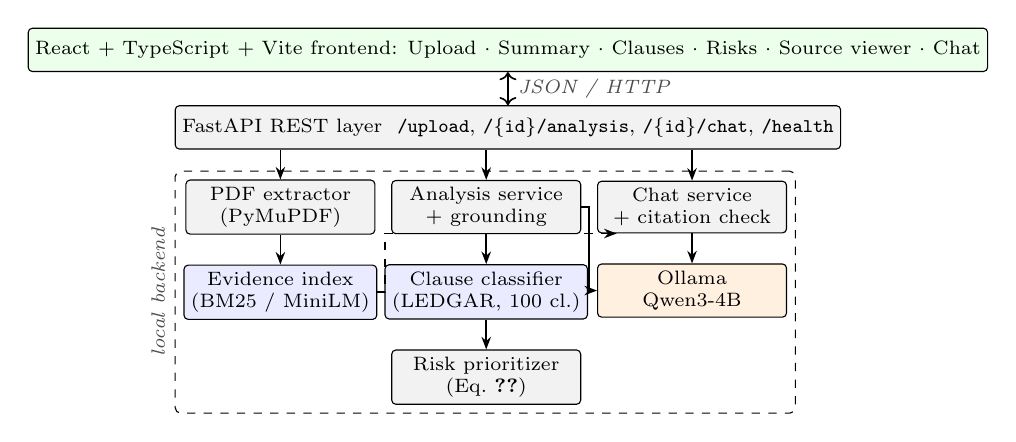
\begin{tikzpicture}[node distance=0.32cm and 0.3cm]
\node[ui, minimum width=7.9cm] (fe) {React + TypeScript + Vite frontend: Upload $\cdot$ Summary $\cdot$ Clauses $\cdot$ Risks $\cdot$ Source viewer $\cdot$ Chat};
\node[det, below=0.42cm of fe, minimum width=7.9cm] (api) {FastAPI REST layer \ \texttt{/upload}, \texttt{/\{id\}/analysis}, \texttt{/\{id\}/chat}, \texttt{/health}};
\node[det, below left=0.38cm and -2.55cm of api, minimum width=2.4cm] (pdf) {PDF extractor\\(PyMuPDF)};
\node[det, right=0.2cm of pdf, minimum width=2.4cm] (ana) {Analysis service\\+ grounding};
\node[det, right=0.2cm of ana, minimum width=2.4cm] (chat) {Chat service\\+ citation check};
\node[ml, below=0.38cm of pdf, minimum width=2.4cm] (idx) {Evidence index\\(BM25 / MiniLM)};
\node[ml, below=0.38cm of ana, minimum width=2.4cm] (cls) {Clause classifier\\(LEDGAR, 100 cl.)};
\node[llm, below=0.38cm of chat, minimum width=2.4cm] (oll) {Ollama\\Qwen3-4B};
\node[det, below=0.38cm of cls, minimum width=2.4cm] (risk) {Risk prioritizer\\(Eq.~\ref{eq:risk})};
\draw[arr,<->] (fe) -- node[right,lbl]{JSON / HTTP} (api);
\draw[arr] (api.south -| pdf) -- (pdf);
\draw[arr] (api.south -| ana) -- (ana);
\draw[arr] (api.south -| chat) -- (chat);
\draw[arr] (pdf) -- (idx);
\draw[arr] (ana) -- (cls);
\draw[arr] (ana.east) -- ++(0.1,0) |- (oll.west);
\draw[arr] (chat) -- (oll);
\draw[arr] (cls) -- (risk);
\draw[arr,dashed] (idx.east) -- ++(0.1,0) |- ($(chat.south west)+(0.25,0)$);
\begin{scope}[on background layer]
\node[grp, fit=(pdf)(chat)(idx)(oll)(risk), label={[lbl]left:\rotatebox{90}{local backend}}] {};
\end{scope}
\end{tikzpicture}}
\caption{Overall LexiGuard AI architecture. All components run on the user's workstation; the dashed path is used only in the experimental retrieval QA mode.}
\label{fig:arch}
\end{figure}

\subsection{PDF Processing Pipeline}
PyMuPDF extracts plain text per page, preserving page numbers and word counts; non-PDF and oversize ($>$50\,MB) uploads are rejected. For segmentation, pages are concatenated into a single string $T$ while a character-to-page map $\pi(\cdot)$ is recorded, so that any character offset can be traced to its page. Two regular-expression passes detect numbered clause headings (e.g., ``3.~Payment Obligations'', ``Section 4.2:''): a line-anchored pass for headings on their own line and an inline pass for headings following a sentence break. Each clause spans from its heading to the next heading, and its page range is $[\pi(s),\pi(e-1)]$, where $s$ and $e$ are its start and end offsets. Clauses that cross page boundaries are therefore reported with spans such as ``p.~1--2''. If no headings are found, the system falls back to paragraph chunks.

\subsection{Clause Classification}
Each clause $c$ is truncated to 512 tokens and passed to the classifier, which outputs logits $\mathbf{z}\in\mathbb{R}^{K}$ over $K=100$ LEDGAR categories:
\begin{equation}
p(y=j\mid c)=\frac{\exp(z_j)}{\sum_{k=1}^{K}\exp(z_k)},\qquad \hat{y}=\arg\max_j p(y=j\mid c).
\end{equation}
The top-3 labels and scores are retained for display. The classifier's role is limited to labelling clauses; it does not produce risks, summaries, or answers.

\subsection{Contract Risk Analysis}
The full page-tagged contract is sent to Qwen3-4B with a JSON schema requesting an overview, parties, contract type, dates, key obligations, and a list of risks. Each risk carries a severity, a \emph{finding category} (\texttt{contractual\_defect}, \texttt{negotiation\_point}, or \texttt{informational}), an explanation, and a verbatim \texttt{relevantText} quote. The prompt instructs the model to ground findings only in the supplied text and not to treat the absence of optional clauses as a defect.

\textit{Evidence grounding.} Let $\nu(\cdot)$ map a string to its lowercase alphanumeric token sequence. A quote $q$ is verified if it has at least 15 characters and three tokens and
\begin{equation}
\nu(q)\sqsubseteq\nu(P_i)\ \text{for some page } i,\ \text{or}\ \nu(q)\sqsubseteq\nu(c)\ \text{for some clause } c,
\label{eq:ground}
\end{equation}
where $\sqsubseteq$ denotes contiguous substring containment; a third check over the concatenated document detects quotes that cross a page boundary. Verified quotes inherit the page span of the matching clause; failures set an \texttt{evidence\_unverified} flag.

\textit{Prioritization.} Each finding receives a deterministic score
\begin{equation}
R=100\cdot\left(w_S S+w_F F+w_O O\right)\cdot E,
\label{eq:risk}
\end{equation}
with $w_S=0.45$, $w_F=0.30$, $w_O=0.25$. $S\in\{0.25,0.5,0.75,1.0\}$ encodes LLM severity (low to critical); $F\in[0.2,1]$ is financial exposure, assigned by the first matching pattern group (e.g., uncapped liability 1.0, indemnity 0.85, penalties or interest 0.70); $O\in[0.25,0.9]$ is obligation asymmetry (e.g., sole discretion or no cure right 0.90, short procedural windows 0.75); and $E\in[0.3,1]$ is an evidence multiplier (1.0 for a verified, page-attributed quote; 0.5 for an unverifiable quote; 0.3 for none). Scores map to tiers URGENT ($\geq$70), HIGH ($\geq$45), MODERATE ($\geq$25), and LOW. A per-factor rationale is returned so that the user can see why a finding ranks where it does.

\textit{Obligations and missing information.} LLM-proposed obligations are kept only if they occur in the text. Otherwise, sentences containing binding modals (\emph{shall}, \emph{must}, \ldots) are scored by additive pattern weights (payment terms +4, termination/cure +4, security incidents +4, numeric deadlines +3, service levels +3, etc.) and the top five are shown. Summary fields that cannot be confirmed in the text are reported as ``Not explicitly specified'' rather than filled with defaults, and the chat prompt requires an explicit statement when the document lacks an answer.

\subsection{Evidence Retrieval}
At upload, an evidence index stores each clause (split into windows of at most 1{,}500 characters) with its page span. In the experimental retrieval mode, a question $Q$ is ranked by Okapi BM25 \cite{robertson2009} ($k_1=1.5$, $b=0.75$) and by cosine similarity of all-MiniLM-L6-v2 embeddings \cite{reimers2019}. The two rankings are fused by RRF \cite{cormack2009}:
\begin{equation}
\mathrm{RRF}(d)=\sum_{m\in\{\mathrm{bm25},\mathrm{dense}\}}\frac{1}{k+r_m(d)},\quad k=60,
\end{equation}
where $r_m(d)$ is the rank of clause $d$ under ranker $m$ (only ranks within a 20-candidate pool contribute). The pool is optionally reranked with the ms-marco-MiniLM-L-6-v2 cross-encoder \cite{nogueira2019}, and the top $k{=}5$ clauses are packed into a 12{,}000-character context without cutting any clause.

\subsection{LLM-Based Question Answering}
In the default (\emph{baseline}) mode, the prompt contains all pages, each truncated at 3{,}000 characters and delimited by page markers. Qwen3-4B is called with temperature 0.1, thinking disabled, and JSON output containing an \texttt{answer} and a list of \texttt{sources} (page, verbatim excerpt). The system prompt restricts answers to the supplied text, fixes the valid page range, and prescribes the abstention sentence ``The provided document does not contain information regarding [topic].'' Fig.~\ref{fig:qa} summarizes the workflow.

\begin{figure}[t]
\centering
\resizebox{\columnwidth}{!}{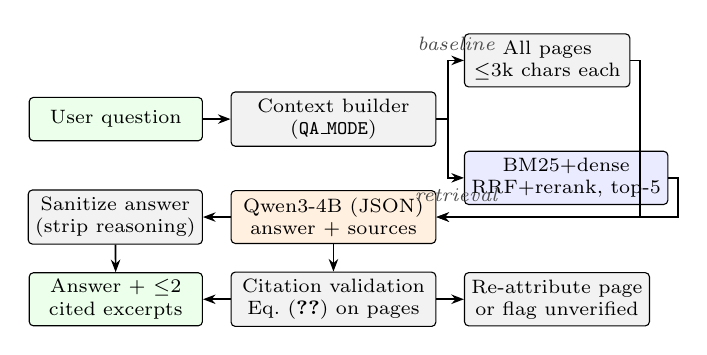
\begin{tikzpicture}[node distance=0.3cm]
\node[ui, minimum width=2.2cm] (q) {User question};
\node[det, right=0.35cm of q, minimum width=2.6cm] (mode) {Context builder\\(\texttt{QA\_MODE})};
\node[det, above right=0.05cm and 0.35cm of mode, minimum width=2.1cm] (base) {All pages\\$\leq$3k chars each};
\node[ml, below right=0.05cm and 0.35cm of mode, minimum width=2.1cm] (ret) {BM25+dense\\RRF+rerank, top-5};
\node[llm, below=0.55cm of mode, minimum width=2.6cm] (llm) {Qwen3-4B (JSON)\\answer + sources};
\node[det, left=0.35cm of llm, minimum width=2.2cm] (clean) {Sanitize answer\\(strip reasoning)};
\node[det, below=0.35cm of llm, minimum width=2.6cm] (val) {Citation validation\\Eq.~\eqref{eq:ground} on pages};
\node[det, right=0.35cm of val, minimum width=2.1cm] (fix) {Re-attribute page\\or flag unverified};
\node[ui, left=0.35cm of val, minimum width=2.2cm] (out) {Answer + $\le$2\\cited excerpts};
\draw[arr] (q) -- (mode);
\draw[arr] (mode.east) -- ++(0.15,0) |- (base.west) node[pos=0.75,above,lbl]{baseline};
\draw[arr] (mode.east) -- ++(0.15,0) |- (ret.west) node[pos=0.75,below,lbl]{retrieval};
\draw[arr] (base.east) -- ++(0.12,0) |- (llm.east);
\draw[arr] (ret.east) -- ++(0.12,0) |- (llm.east);
\draw[arr] (llm) -- (clean);
\draw[arr] (llm) -- (val);
\draw[arr] (val) -- (fix);
\draw[arr] (val) -- (out);
\draw[arr] (clean) -- (out);
\end{tikzpicture}}
\caption{Question-answering workflow with deterministic citation verification. The baseline mode is the deployed default; the retrieval mode is experimental.}
\label{fig:qa}
\end{figure}

\subsection{Citation and Evidence Presentation}
For each returned source, the system drops citations to nonexistent pages, tests Eq.~\eqref{eq:ground} against the cited page, and, if that fails, searches all pages and re-attributes the citation to the page where the excerpt actually occurs. Each source is marked \texttt{excerpt\_verified}; duplicates are removed and at most two distinct excerpts are shown. In the interface, clause and risk cards display page spans; selecting one opens the source viewer at the corresponding page anchor. Category and severity are rendered as separate badges.

\section{Implementation and System Integration}
Table~\ref{tab:stack} lists the components and their responsibilities.

\begin{table}[t]
\caption{Technology Stack and Component Responsibilities}
\label{tab:stack}
\centering
\footnotesize
\setlength{\tabcolsep}{3pt}
\begin{tabular}{@{}>{\raggedright}p{2.0cm}>{\raggedright}p{2.3cm}p{3.9cm}@{}}
\toprule
\textbf{Component} & \textbf{Technology} & \textbf{Responsibility} \\
\midrule
Frontend & React 18, TypeScript, Vite, Tailwind CSS & Upload, analysis tabs, source viewer, chat; Vitest tests \\
Backend & Python, FastAPI, Pydantic v2 & REST endpoints, in-memory store, orchestration; pytest tests \\
PDF extraction & PyMuPDF & Per-page text, page/word counts \\
Clause classifier & LiTiL Clause Classifier (ModernBERT-large) & 100-class LEDGAR label + top-3 scores per clause \\
LLM & Qwen3-4B \cite{qwen2025} via Ollama & Summary, risks, obligations, answers (JSON) \\
Retrieval (exp.) & BM25; all-MiniLM-L6-v2; ms-marco cross-encoder & Clause ranking for retrieval QA mode \\
Verification & Python (regex, token matching) & Quote grounding, page re-attribution, risk score \\
\bottomrule
\end{tabular}
\end{table}

\textit{Frontend.} The React application provides upload, dashboard, history, settings, and an analysis page with Summary, Clauses, Risks, and Source tabs plus a chat panel. A typed API client calls the backend; a health hook reports backend availability.

\textit{Backend.} FastAPI exposes, under \texttt{/api/documents}, the endpoints \texttt{POST /upload}, \texttt{GET /\{id\}}, \texttt{GET /\{id\}/analysis}, \texttt{POST /\{id\}/chat}, and \texttt{DELETE /\{id\}}, plus \texttt{GET /api/health}. Timeouts map to HTTP 504 and processing errors to HTTP 500, so failures are never reported as successful analyses. A configuration flag selects a deterministic demonstration mode or live AI mode.

\textit{Clause classifier.} The deployed checkpoint is \path{litillabs/litil-clause-classifier}, obtained from Hugging Face. Its configuration declares a \texttt{ModernBertForSequenceClassification} head; the model card states it is ModernBERT-large \cite{warner2024} fine-tuned on the 60{,}000 LEDGAR training provisions of LexGLUE \cite{chalkidis2022}. It is loaded once per process from a local directory and run on CPU in float32. A separate DeBERTa-v3-base \cite{he2023} fine-tuning pipeline was also developed in the project (Section~\ref{sec:lim}).

\textit{Qwen3 local inference.} An asynchronous client calls Ollama's \texttt{/api/generate} with \texttt{format=json}, temperature 0.1--0.2, prediction limits of 512--1{,}024 tokens, and a 120\,s timeout. Truncated JSON is repaired by appending closing brackets, and placeholder or schema-echo values are discarded.

\textit{Data flow.} Upload triggers extraction and indexing; analysis runs segmentation $\rightarrow$ classification $\rightarrow$ LLM analysis $\rightarrow$ grounding $\rightarrow$ summary repair $\rightarrow$ prioritization (Fig.~\ref{fig:flow}); chat runs the workflow in Fig.~\ref{fig:qa}.

\begin{figure}[t]
\centering
\resizebox{\columnwidth}{!}{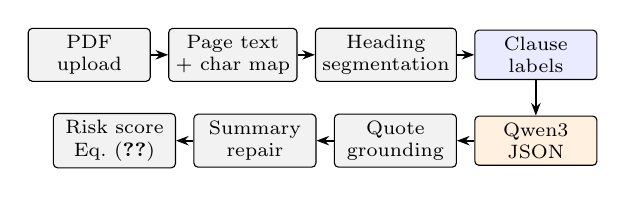
\begin{tikzpicture}[node distance=0.22cm]
\node[det, minimum width=1.55cm] (a) {PDF\\upload};
\node[det, right=of a, minimum width=1.55cm] (b) {Page text\\+ char map};
\node[det, right=of b, minimum width=1.55cm] (c) {Heading\\segmentation};
\node[ml, right=of c, minimum width=1.55cm] (d) {Clause\\labels};
\node[llm, below=0.45cm of d, minimum width=1.55cm] (e) {Qwen3\\JSON};
\node[det, left=of e, minimum width=1.55cm] (f) {Quote\\grounding};
\node[det, left=of f, minimum width=1.55cm] (g) {Summary\\repair};
\node[det, left=of g, minimum width=1.55cm] (h) {Risk score\\Eq.~\eqref{eq:risk}};
\draw[arr] (a)--(b); \draw[arr] (b)--(c); \draw[arr] (c)--(d); \draw[arr] (d)--(e);
\draw[arr] (e)--(f); \draw[arr] (f)--(g); \draw[arr] (g)--(h);
\end{tikzpicture}}
\caption{End-to-end analysis pipeline from upload to prioritized findings.}
\label{fig:flow}
\end{figure}

\section{Results and Discussion}
\subsection{Implementation Screenshots}
Figs.~\ref{fig:sum}--\ref{fig:chat} show the running system in AI mode on a two-page fictional software services agreement (706 extracted words). The summary (Fig.~\ref{fig:sum}) reports parties, type, effective date, term, and five key obligations, all present verbatim in the contract. The clause view (Fig.~\ref{fig:cls}) shows LEDGAR labels and the page span ``Page 1--2'' for a clause that crosses a page break; it also shows a misclassification (the limitation-of-liability clause labelled \emph{Survival}), which illustrates why labels are presented as aids rather than ground truth. The risk view (Fig.~\ref{fig:risk}) separates finding category from severity, shows the verified quote, the clause and page, and the priority score of Eq.~\eqref{eq:risk}. The chat panel (Fig.~\ref{fig:chat}) answers a payment question with a verified page-1 citation.

\begin{figure}[t]
\centering
\includegraphics[width=\columnwidth]{fig_summary.png}
\caption{Executive summary: LLM output repaired and validated against the source text.}
\label{fig:sum}
\end{figure}

\begin{figure}[t]
\centering
\includegraphics[width=\columnwidth]{fig_clauses.png}
\caption{Clause view with predicted LEDGAR categories and page spans, including a cross-page clause (p.~1--2).}
\label{fig:cls}
\end{figure}

\begin{figure*}[t]
\centering
\includegraphics[width=0.82\textwidth]{fig_risk.png}
\caption{Risk analysis view: finding category (Defect, Informational, Negotiation Point), severity, source clause and page, verified quotation, and explainable priority score.}
\label{fig:risk}
\end{figure*}

\begin{figure}[t]
\centering
\includegraphics[width=\columnwidth]{fig_chat.png}
\caption{Document-grounded question answering with a verified page-level citation.}
\label{fig:chat}
\end{figure}

\subsection{Datasets}
Table~\ref{tab:data} lists the data used. The two synthetic contracts and the seed set were authored for testing; LegalBench-RAG and ContractNLI carry expert annotations.

\begin{table}[t]
\caption{Datasets Used in Development and Evaluation}
\label{tab:data}
\centering
\footnotesize
\setlength{\tabcolsep}{3pt}
\begin{tabular}{@{}>{\raggedright}p{2.1cm}>{\raggedright}p{2.9cm}p{3.2cm}@{}}
\toprule
\textbf{Dataset} & \textbf{Size used} & \textbf{Purpose} \\
\midrule
LEDGAR (LexGLUE) \cite{tuggener2020,chalkidis2022} & 60k/10k/10k, 100 classes & Classifier training (by provider) \\
LegalBench-RAG \cite{pipitone2024} & 200 Q, 18 docs (50 each: ContractNLI, CUAD, MAUD, PrivacyQA) & Retrieval evaluation \\
ContractNLI \cite{koreeda2021} & Test split, 30 docs $\times$ 17 hyp.\ = 510 Q (291 answerable) & Retrieval, abstention signal \\
Seed set & 2 synthetic contracts, 25 Q & Pipeline and chat check \\
Synthetic PDFs & 2-page MSA; 1-page memo & Functional tests \\
\bottomrule
\end{tabular}
\end{table}

\subsection{Clause Classification}
No clause-classification experiment was run within this project on the deployed model; the training, checkpoint, and log directories of the in-house DeBERTa pipeline are empty, so its results are not reported. For reference only, the provider's model card reports 88.82\% accuracy and 83.17\% macro-F1 on the 10{,}000-provision LEDGAR \emph{test} split. These figures are the provider's claims and were not reproduced here. The metrics are defined as
\begin{equation}
\mathrm{Acc}=\frac{1}{N}\sum_{i=1}^{N}\mathbb{1}[\hat{y}_i=y_i],\qquad \mathrm{F1}_{\mathrm{macro}}=\frac{1}{K}\sum_{j=1}^{K}\frac{2P_jR_j}{P_j+R_j},
\end{equation}
where $P_j$ and $R_j$ are the precision and recall of class $j$ over $N$ samples.

\subsection{Functional Testing}
The project's validation report records 111/111 passing backend tests (pytest) and 8/8 frontend tests (Vitest), together with live runs of Ollama and the classifier on two synthetic PDFs. Table~\ref{tab:func} condenses the outcomes. All 16 recorded cases passed, including the cross-page span of the liability clause (p.~1--2), the separation of an omitted payment deadline (defect) from a 1.5\%/month interest rate (negotiation point), and explicit abstention on absent patent terms. One defect was found and fixed: PyMuPDF line breaks inside quoted sentences caused correct excerpts to fail exact matching, which motivated the token normalization $\nu(\cdot)$ in Eq.~\eqref{eq:ground}.

\begin{table}[t]
\caption{Functional Test Cases on Synthetic Contracts}
\label{tab:func}
\centering
\footnotesize
\setlength{\tabcolsep}{3pt}
\begin{tabular}{@{}>{\raggedright}p{2.7cm}>{\raggedright}p{4.2cm}c@{}}
\toprule
\textbf{Test group} & \textbf{Observed output (abridged)} & \textbf{Result} \\
\midrule
Segmentation, MSA (TC-1.1) & 7 clauses; clause 5 tagged p.~1--2 & Pass \\
Key obligations (TC-1.2) & USD 25{,}000 fee in 30 days; 1.5\% interest; 24\,h incident notice; 15-min response & Pass \\
Risk categories (TC-1.3) & 1 defect, 1 negotiation point, 1 informational & Pass \\
Factual QA (TC-1.4--1.8) & Payment, incident, SLA, cure, cap + law (cross-page) answered with verified citations & 5/5 \\
Absence, MSA (TC-1.9) & ``does not contain information regarding patent licensing'' & Pass \\
Incomplete memo (TC-2.1--2.3) & Obligations extracted; missing deadlines as defects; no-cure termination as negotiation point & 3/3 \\
Missing-term QA (TC-2.4--2.7) & Absence of payment date, incident window, SLA, cure period disclosed & 4/4 \\
\bottomrule
\end{tabular}
\end{table}

\subsection{Evidence Retrieval Evaluation}
The retrieval mode was evaluated with a dedicated harness under \emph{within-document} retrieval: each question searches only its own contract, so results are not comparable with LegalBench-RAG's corpus-level setting. A gold span counts as retrieved when the top-$k$ clauses cover at least 50\% of it, and
\begin{equation}
\mathrm{complete@}k=\frac{1}{|\mathcal{Q}|}\sum_{Q\in\mathcal{Q}}\mathbb{1}\!\left[G_Q\subseteq\mathrm{Top}_k(Q)\right],
\end{equation}
where $G_Q$ is the set of gold spans of question $Q$. Character precision@$k$ is the fraction of retrieved characters that belong to gold spans. Table~\ref{tab:ret} reports results at $k=5$.

\begin{table}[t]
\caption{Within-Document Retrieval, complete@5 (Answerable Questions)}
\label{tab:ret}
\centering
\footnotesize
\setlength{\tabcolsep}{4pt}
\begin{tabular}{@{}lcccc@{}}
\toprule
\textbf{Dataset ($n$)} & \textbf{BM25} & \textbf{Dense} & \textbf{Hybrid} & \textbf{Hyb.+rerank} \\
\midrule
LegalBench-RAG (200) & 0.795 & 0.710 & 0.805 & 0.810 \\
\quad CUAD subset (50) & 0.80 & -- & 0.84 & 0.96 \\
\quad MAUD subset (50) & 0.46 & -- & 0.46 & 0.34 \\
ContractNLI (291) & \textbf{0.894} & 0.839 & 0.887 & 0.866 \\
\midrule
Char.\ prec.@5, LB-RAG & 0.063 & 0.062 & 0.061 & 0.064 \\
\bottomrule
\end{tabular}
\end{table}

Three observations follow. First, one-shot retrieval misses complete evidence for roughly one in five LegalBench-RAG and one in eight ContractNLI questions. Second, the general-domain reranker helps on CUAD but is below BM25 alone on ContractNLI and degrades MAUD, so it is not clearly beneficial for contracts. Third, low character precision ($\approx$0.06) shows that oversized clauses inflate coverage: the heading-based segmenter produced only 2 clauses for one 313k-character MAUD merger agreement. In addition, the top-1 retrieval score separated answerable from \emph{NotMentioned} ContractNLI questions with AUROC of only 0.60 (BM25), 0.66 (dense), and 0.67 (cross-encoder), indicating that a score threshold is an unreliable abstention signal. Only retrieval was measured on these sets; no significance tests were run, and MAUD's 50 questions come from four agreements.

\subsection{Question Answering and Citation Checks}
On the 25-question seed set, both QA modes were run end to end with Ollama. Heuristic checks (not correctness grades) found that answerable questions whose citations hit a gold page numbered 19/20 in baseline mode and 20/20 in retrieval mode, and that unanswerable questions were abstained on in 3/5 and 5/5 cases, respectively; mean latency was 9.18\,s and 7.31\,s per question on the development workstation. In the baseline prompt, 25 of 26 gold items survived the 3{,}000-character page cut. These figures come from two small synthetic contracts and demonstrate pipeline behaviour, not general superiority of either mode; manual correctness grading remains to be completed.

\section{Limitations and Future Work}
\label{sec:lim}
\textit{Model provenance.} The deployed classifier is a third-party ModernBERT checkpoint whose reported test metrics were not independently reproduced. The in-house DeBERTa-v3-base pipeline (lr $10^{-5}$, effective batch 16, 3 epochs, 512 tokens) has no retained logs or checkpoints, and previously quoted validation figures could not be reconciled with any stored record; they are therefore omitted. Re-running and archiving that experiment, and evaluating the deployed model on held-out data, are first priorities.

\textit{Analysis scope.} Baseline QA truncates pages at 3{,}000 characters, so long pages can lose evidence; risk severity and categories originate from a 4B LLM and are not validated by legal experts; the financial and asymmetry factors are keyword-based; the document store is in memory; scanned PDFs (no OCR) are unsupported. No user study, expert evaluation, or hallucination-rate measurement has been performed.

\textit{Future work.} Planned work includes size-capped clause segmentation, a legal-domain reranker, and a failure-aware evidence controller that checks per-requirement evidence sufficiency and performs targeted second-round retrieval, compared against the B1 baseline reported here; a proposed risk-aware retrieval variant is also under consideration as separate research. Expert-graded evaluation of summaries, risk findings, and answers is required before any claim of answer quality.

\section{Conclusion}
LexiGuard AI demonstrates that a contract analysis assistant can run entirely on a local workstation by combining a 100-class LEDGAR clause classifier, a small local LLM, and deterministic verification. Its principal design choice is that model output is not displayed as evidence until code has matched it to the source text and attributed it to a page; unverified quotations are flagged and lower a finding's priority score. Functional tests confirm the intended behaviour on synthetic contracts, and the retrieval study quantifies where one-shot clause retrieval falls short on expert-annotated data. The system supports document orientation and does not constitute legal advice.

\begin{thebibliography}{99}
\footnotesize
\bibitem{vaswani2017} A. Vaswani \textit{et al.}, ``Attention is all you need,'' in \textit{Proc. NeurIPS}, 2017, pp. 5998--6008.
\bibitem{devlin2019} J. Devlin, M.-W. Chang, K. Lee, and K. Toutanova, ``BERT: Pre-training of deep bidirectional transformers for language understanding,'' in \textit{Proc. NAACL-HLT}, 2019, pp. 4171--4186.
\bibitem{tuggener2020} D. Tuggener, P. von D\"aniken, T. Peetz, and M. Cieliebak, ``LEDGAR: A large-scale multi-label corpus for text classification of legal provisions in contracts,'' in \textit{Proc. LREC}, 2020, pp. 1235--1241.
\bibitem{chalkidis2022} I. Chalkidis \textit{et al.}, ``LexGLUE: A benchmark dataset for legal language understanding in English,'' in \textit{Proc. ACL}, 2022, pp. 4310--4330.
\bibitem{ji2023} Z. Ji \textit{et al.}, ``Survey of hallucination in natural language generation,'' \textit{ACM Comput. Surv.}, vol. 55, no. 12, pp. 1--38, 2023.
\bibitem{magesh2024} V. Magesh, F. Surani, M. Dahl, M. Suzgun, C. D. Manning, and D. E. Ho, ``Hallucination-free? Assessing the reliability of leading AI legal research tools,'' arXiv:2405.20362, 2024.
\bibitem{zhong2020} H. Zhong, C. Xiao, C. Tu, T. Zhang, Z. Liu, and M. Sun, ``How does NLP benefit legal system: A summary of legal artificial intelligence,'' in \textit{Proc. ACL}, 2020, pp. 5218--5230.
\bibitem{hendrycks2021} D. Hendrycks, C. Burns, A. Chen, and S. Ball, ``CUAD: An expert-annotated NLP dataset for legal contract review,'' in \textit{Proc. NeurIPS Datasets and Benchmarks Track}, 2021.
\bibitem{koreeda2021} Y. Koreeda and C. D. Manning, ``ContractNLI: A dataset for document-level natural language inference for contracts,'' in \textit{Findings of EMNLP}, 2021, pp. 1907--1919.
\bibitem{guha2023} N. Guha \textit{et al.}, ``LegalBench: A collaboratively built benchmark for measuring legal reasoning in large language models,'' in \textit{Proc. NeurIPS Datasets and Benchmarks Track}, 2023.
\bibitem{he2021} P. He, X. Liu, J. Gao, and W. Chen, ``DeBERTa: Decoding-enhanced BERT with disentangled attention,'' in \textit{Proc. ICLR}, 2021.
\bibitem{he2023} P. He, J. Gao, and W. Chen, ``DeBERTaV3: Improving DeBERTa using ELECTRA-style pre-training with gradient-disentangled embedding sharing,'' in \textit{Proc. ICLR}, 2023.
\bibitem{warner2024} B. Warner \textit{et al.}, ``Smarter, better, faster, longer: A modern bidirectional encoder for fast, memory efficient, and long context finetuning and inference,'' arXiv:2412.13663, 2024.
\bibitem{lewis2020} P. Lewis \textit{et al.}, ``Retrieval-augmented generation for knowledge-intensive NLP tasks,'' in \textit{Proc. NeurIPS}, 2020, pp. 9459--9474.
\bibitem{robertson2009} S. Robertson and H. Zaragoza, ``The probabilistic relevance framework: BM25 and beyond,'' \textit{Found. Trends Inf. Retr.}, vol. 3, no. 4, pp. 333--389, 2009.
\bibitem{reimers2019} N. Reimers and I. Gurevych, ``Sentence-BERT: Sentence embeddings using Siamese BERT-networks,'' in \textit{Proc. EMNLP-IJCNLP}, 2019, pp. 3982--3992.
\bibitem{nogueira2019} R. Nogueira and K. Cho, ``Passage re-ranking with BERT,'' arXiv:1901.04085, 2019.
\bibitem{cormack2009} G. V. Cormack, C. L. A. Clarke, and S. B\"uttcher, ``Reciprocal rank fusion outperforms Condorcet and individual rank learning methods,'' in \textit{Proc. ACM SIGIR}, 2009, pp. 758--759.
\bibitem{pipitone2024} N. Pipitone and G. H. Alami, ``LegalBench-RAG: A benchmark for retrieval-augmented generation in the legal domain,'' arXiv:2408.10343, 2024.
\bibitem{gao2023} T. Gao, H. Yen, J. Yu, and D. Chen, ``Enabling large language models to generate text with citations,'' in \textit{Proc. EMNLP}, 2023, pp. 6465--6488.
\bibitem{qwen2025} Qwen Team, ``Qwen3 technical report,'' arXiv:2505.09388, 2025.
\end{thebibliography}

\end{document}
